\begin{figure}
\centering

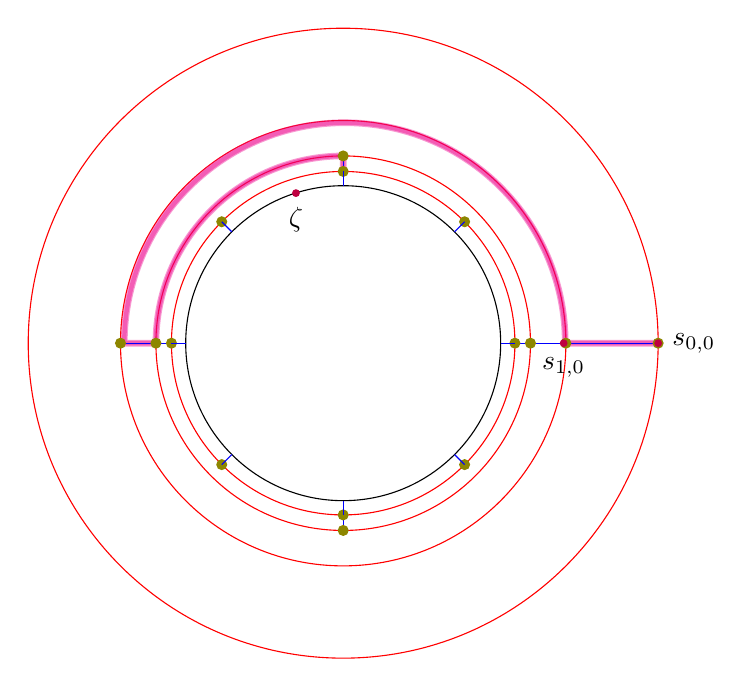
\begin{tikzpicture}[scale=2]
		
		
\draw (0,0) circle (1);
\draw[red] (0,0) circle (2);
	\draw[red] (0,0) circle (2^0.5);
	\draw[red] (0,0) circle (2^0.25);
	\draw[red] (0,0) circle (2^0.125);


\draw [magenta,-,
	double=magenta,
	double distance=4\pgflinewidth, opacity=0.4,
	] (2,0) -- (1.41,0) arc (0:180:1.4) -- (-1.189,0) arc (180:90:1.189) -- (0,1.0905);
\draw[blue] (2,0);

\draw[blue] (2,0) --  (1,0);	
\draw[blue] (-2^0.5,0) -- (-1,0);	
\draw[blue] (0, 2^0.25) -- (0,1);	
\draw[blue] (0, -2^0.25) -- (0,-1);	

\fill[olive] (2,0) circle (1pt);
\fill[olive] (2^0.5,0) circle (1pt);
\fill[olive] (-2^0.5,0) circle (1pt);

\foreach \angle in {0,90,180,270}
\fill[olive] (\angle:2^0.25) circle (1pt);

\foreach \angle in {0,45,90,135,180,225,270,315}
\fill[olive] (\angle:2^0.125) circle (1pt);
\foreach \angle in {0,45,90,135,180,225,270,315} 		
\draw[blue] (\angle:2^0.125) -- (\angle:1);


\node[circle,inner sep=1pt,fill=purple,label=below:{$\zeta$}] at (-0.3,0.953) {};

\node[circle,inner sep=1pt,fill=purple,label=right:{$s_{0,0}$}] at (2,0) {};

\node[circle,inner sep=1pt,fill=purple,label=below:{$s_{1,0}$}] at (1.4,0) {};

\end{tikzpicture}

\caption{The central itinerary to a point $\zeta$. 
	%Carleson box decomposition of $\mathbb D^*$.
} \label{fig:Carleson1}
\end{figure}

